\section{Continuous functions}

A function \(f\) maps elements of a set \(A\) to elements of another set \(B\). We denote this as \(f : A \rightarrow B\). In practice, most functions we consider will have type \(\mathbb{R} \rightarrow \mathbb{R}\).

If a function maps a number \(x\) to its square \(x^2\), we can denote this by \(x \mapsto x^2\). (Note the difference in the arrow symbol used --- the symbol \(\mapsto\) is read as ``maps to''.)

A function \(y = f(x)\) can be represented graphically as the set of points \((x, y)\). See figure \ref{fig:Ch02-quadratic-graph}.

\begin{figure}[H]
    \centering

    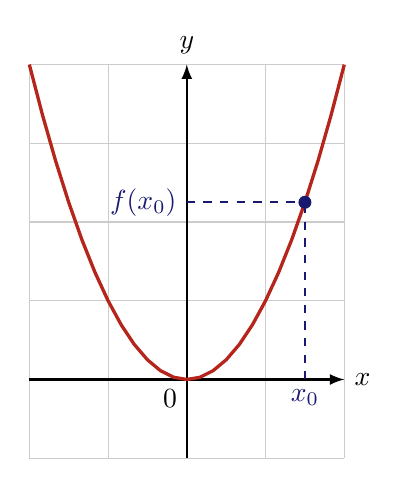
\begin{tikzpicture}
        \draw[thin,gray!40] (-2,-1) grid (2, 4);
        \draw[thick, ->, >=latex] (-2,0)--(2,0) node[right]{\(x\)};
        \draw[thick, ->, >=latex] (0,-1)--(0,4) node[above]{\(y\)};
        \draw (0, 0) node[below left] {0};

        \draw [BrickRed, very thick, domain=-2:2] plot (\x, {\x*\x}); 

        \draw[MidnightBlue, dashed, thick] (1.5, 0) node[below]{\(x_0\)} --(1.5, 2.25);
        \draw[MidnightBlue, dashed, thick] (0, 2.25) node[left]{\(f(x_0)\)} --(1.5, 2.25);

        \filldraw[radius=0.075, MidnightBlue] (1.5,2.25) circle;
    \end{tikzpicture}
    
    \caption{The graph of the function \(y = x^2\).}
    \label{fig:Ch02-quadratic-graph}
\end{figure}

In the next few subsections, we will be looking at some classic mathematical functions.


\subsection{Trigonometric functions}

Consider a point \(P\) on the unit circle. If we let \(\theta\) be the angle between \(OP\) and the horizontal axis, then the coordinates of \(P\) can be expressed as \((\cos{\theta},\; \sin{\theta})\). This is illustrated in figure \ref{fig:Ch02-trig-funcs-on-unit-circle}.

\begin{figure}[H]
    \centering

    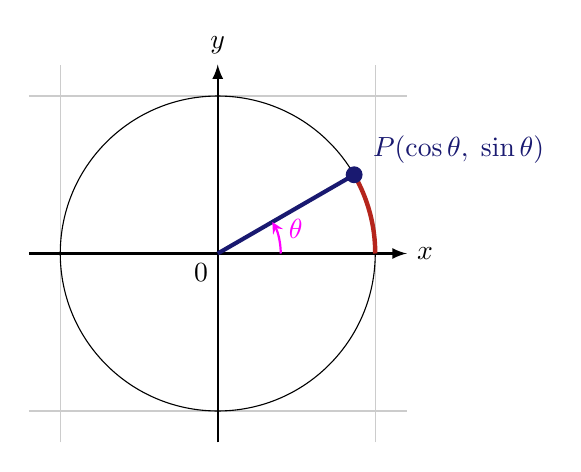
\begin{tikzpicture}[scale=2]
        \draw[thin,gray!40] (-1.2,-1.2) grid (1.2, 1.2);

        \draw[radius=1] (0, 0) circle;

        \draw[thick, ->, >=latex] (-1.2,0)--(1.2,0) node[right]{\(x\)};
        \draw[thick, ->, >=latex] (0,-1.2)--(0,1.2) node[above]{\(y\)};
        \draw (0, 0) node[below left] {\(0\)};

        \draw[BrickRed, ultra thick] (1, 0) arc (0:30:1);

        \filldraw[radius=0.05, MidnightBlue] ({sqrt(3)/2}, 0.5) circle;
        \draw[line width=1.5pt, MidnightBlue] (0,0)--({sqrt(3)/2}, 0.5) node[anchor=south west]{\(\;P(\cos{\theta},\; \sin{\theta})\)};
        \draw[-stealth,Fuchsia, thick] (0.4, 0) arc (0:30:0.4) node[pos=0.5, anchor=west, shift={(0, 0.1)}]{\(\theta\)};

        
    \end{tikzpicture}
    
    \caption{The trigonometric functions \(\cos{\theta}\) and \(\sin{\theta}\) can be defined using the unit circle. Note that if we are measuring \(\theta\) in radians, then the length of the arc highlighted in red must be equal to \(\theta\).}
    \label{fig:Ch02-trig-funcs-on-unit-circle}
\end{figure}

We've previously seen the values of \(\sin{\theta}\) and \(\cos{\theta}\) for some classic angles \(\theta\) in table \ref{tab:Ch01-classic-angle-trig}. Plotting these functions on a graph results in figure \ref{fig:Ch02-trig-funcs-graph}.

\begin{figure}[H]
    \centering

    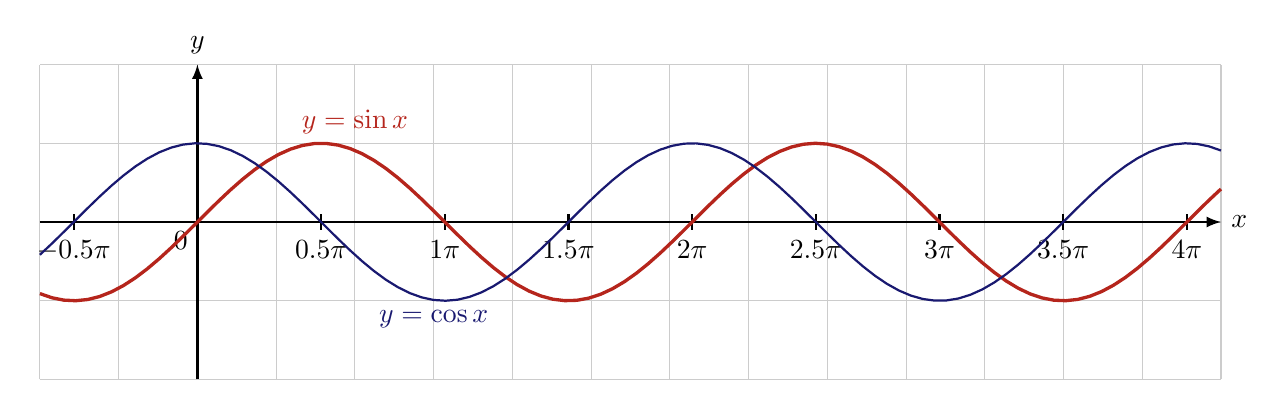
\begin{tikzpicture}
        \draw[thin,gray!40] (-2,-2) grid (13, 2);
        \draw[thick, ->, >=latex] (-2,0)--(13,0) node[right]{\(x\)};
        \draw[thick, ->, >=latex] (0,-2)--(0,2) node[above]{\(y\)};
        \draw (0, 0) node[below left] {0};

        \foreach \x in {-0.5, 0.5, 1, ..., 4} {
            \draw[thick] (\x*3.14159, 0.1) -- (\x*3.14159, -0.1) node[below] {\(\x\pi\)};
        }

        % \x r means to convert '\x' from degrees to radians:
        \draw [BrickRed, very thick, domain=-2:13, samples=100] plot (\x,{sin(\x r)});

        \draw [MidnightBlue, thick, domain=-2:13, samples=100] plot (\x,{cos(\x r)});

        \draw node[BrickRed, above] at (2, 1) {\(y = \sin{x}\)};
        \draw node[MidnightBlue, below] at (3, -1) {\(y = \cos{x}\)};
    \end{tikzpicture}
    
    \caption{The graph of the functions \(\sin{x}\) and \(\cos{x}\).}
    \label{fig:Ch02-trig-funcs-graph}
\end{figure}





\subsection{Exponential and logarithm}

One way to define the exponential function \(\exp\) is as follows.
%
\begin{align*}
    \exp(x + y) &= \exp(x) \cdot \exp(y)\\
    \exp(0) &= 1\\
    \frac{d}{dx} \exp(x) &= \exp(x) 
\end{align*}
%
Note that the first two relationships can be satisfied by any function of the form \(f(x) = a^x\) where \(a \in \mathbb{R}\). However, if we take all three conditions into account, the only function satisfying them is \(\exp(x) = e^x\), where \(e = 2.71828\cdots\) is Euler's number.

The exponential function \(\exp(x) = e^x\) is plotted in figure \ref{fig:Ch02-exp-graph}. Note that:
%
\begin{itemize}
    \item For all values of \(x\), we have \(\exp(x) > 0\).
    \item When \(x\) is negative, \(\exp(x)\) is very small.
    \item The value of \(\exp(x)\) grows very fast as \(x\) increases.
\end{itemize}

\begin{figure}[H]
    \centering

    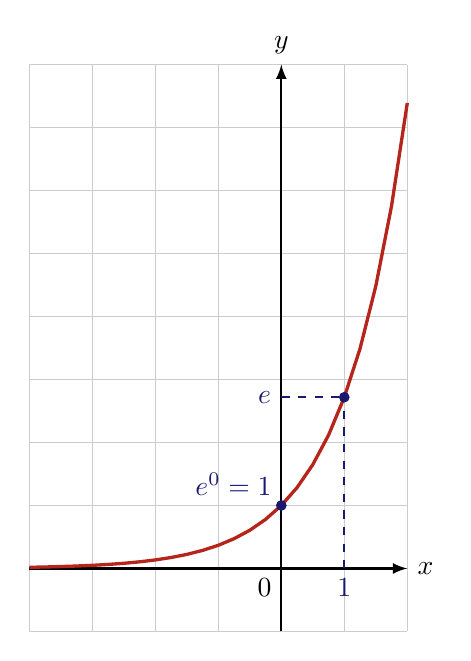
\begin{tikzpicture}[scale=0.8]
        \draw[thin,gray!40] (-4,-1) grid (2, 8);
        \draw[thick, ->, >=latex] (-4,0)--(2,0) node[right]{\(x\)};
        \draw[thick, ->, >=latex] (0,-1)--(0,8) node[above]{\(y\)};
        \draw (0, 0) node[below left] {0};

        \draw [BrickRed, very thick, domain=-4:2] plot (\x, {2.71828^\x}); 
        \filldraw[radius=0.075, MidnightBlue] (0,1) circle node[above left] {\(e^0 = 1\)};

        \draw[MidnightBlue, dashed, thick] (1, 0) node[below]{\(1\)} --(1, 2.71828);
        \draw[MidnightBlue, dashed, thick] (0, 2.71828) node[left]{\(e\)} --(1, 2.71828);

        \filldraw[radius=0.075, MidnightBlue] (1, 2.71828) circle;
    \end{tikzpicture}
    
    \caption{The graph of the function \(y = \exp(x) = e^x\).}
    \label{fig:Ch02-exp-graph}
\end{figure}

The natural logarithm \(\ln{x}\) is the inverse of the exponential, meaning that \(\ln(e^x) = x\). This results in the following properties.
%
\begin{align*}
    \ln(ab) &= \ln{a} + \ln{b}\\
    \ln\left(\frac{a}{b}\right) &= \ln{a} - \ln{b}\\
    \ln{1} &= 0\\
    \ln{e} &= 1\\
    a^x &= e^{x\ln{a}}\\
    \ln(a^x) &= x\ln{a}
\end{align*}
%
Since \(e^x > 0\) for all \(x\), the natural logarithm \(\ln{x}\) is only defined for positive values of \(x\).

The plot of \(y = \ln{x}\) is given in figure \ref{fig:Ch02-ln-graph}. Note that:
%
\begin{itemize}
    \item For \(x < 1\), we have \(\ln{x} < 0\).
    \item The curve intersects the \(x\)-axis at \((1, 0)\).
    \item For \(x > 1\), the value of \(\ln{x}\) grows very slowly as \(x\) increases.
\end{itemize}

\begin{figure}[H]
    \centering

    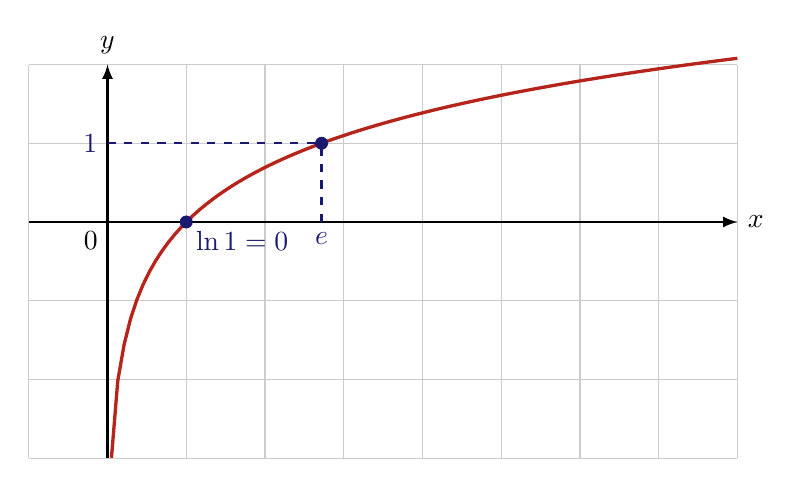
\begin{tikzpicture}
        \draw[thin,gray!40] (-1,-3) grid (8, 2);
        \draw[thick, ->, >=latex] (-1,0)--(8,0) node[right]{\(x\)};
        \draw[thick, ->, >=latex] (0,-3)--(0,2) node[above]{\(y\)};
        \draw (0, 0) node[below left] {0};

        \draw [BrickRed, very thick, domain=0.05:8, samples=100] plot (\x, {ln(\x)}); 
        \filldraw[radius=0.075, MidnightBlue] (1, 0) circle node[below right] {\(\ln{1} = 0\)};

        \draw[MidnightBlue, dashed, thick] (0, 1) node[left]{\(1\)} --(2.71828, 1);
        \draw[MidnightBlue, dashed, thick] (2.71828, 0) node[below]{\(e\)} --(2.71828, 1);

        \filldraw[radius=0.075, MidnightBlue] (2.71828, 1) circle;
    \end{tikzpicture}
    
    \caption{The graph of the function \(y = \exp(x) = e^x\).}
    \label{fig:Ch02-ln-graph}
\end{figure}




\subsection{Introduction to limits}

The idea of limits is simple.
%
\begin{quote}
    As the input \(x\) approaches a value \(p\), the output \(f(x)\) also approaches a value \(L\). (Both \(p\) and \(L\) possibly infinite.) To denote this we write \(f(x) \rightarrow L\) as \(x \rightarrow p\), or \(\lim_{x \rightarrow p} f(x) = L\).
\end{quote}

How do you formally define something like that?

Let us consider the simplest case, where both \(p\) and \(L\) are finite. We give the following definition.
%
\begin{quote}
    \textbf{Definition of a limit, with both \(p\) and \(L\) finite.}

    The main idea is that \(f(x)\) can get \textit{arbitrarily close} to \(L\) as long as \(x\) is close enough to \(p\).

    In other words, {\color{BrickRed} no matter how close we want our output to be to \(L\)}, {\color{Fuchsia} we can always find a range of inputs around \(p\)} such that {\color{MidnightBlue} the output is within that range}. This is written as
    %
    \[
    {\color{BrickRed} \forall \epsilon > 0},\;
    {\color{Fuchsia} \exists \delta > 0},\;
    {\color{Fuchsia} \forall x \in \mathbb{R}},\;
    {\color{Fuchsia} 0 < \abs{x - p} < \delta}
    \Rightarrow
    {\color{MidnightBlue} \abs{f(x) - L} < \epsilon}
    \text{.}
    \]
\end{quote}
%
This is called the epsilon-delta or \((\epsilon, \delta)\) definition of a limit. See figure \ref{fig:Ch02-lim-val-val} for an illustration of this.

\begin{figure}[H]
    \centering

    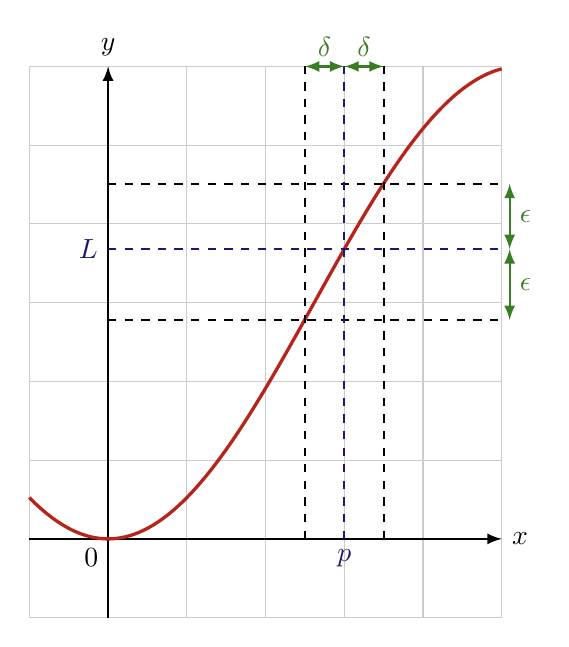
\begin{tikzpicture}
        \draw[thin,gray!40] (-1,-1) grid (5, 6);
        \draw[thick, ->, >=latex] (-1,0)--(5,0) node[right]{\(x\)};
        \draw[thick, ->, >=latex] (0,-1)--(0,6) node[above]{\(y\)};
        \draw (0, 0) node[below left] {0};

        \draw [BrickRed, very thick, domain=-1:5, samples=100] plot (\x, {6*(sin((0.3*\x) r))^2}); 

        \draw[dashed, thick] (0, 2.78) -- (5, 2.78);
        \draw[dashed, thick] (0, 4.51) -- (5, 4.51);

        \draw[dashed, thick] (2.5, 0) -- (2.5, 6);
        \draw[dashed, thick] (3.5, 0) -- (3.5, 6);

        \draw[MidnightBlue, dashed, thick] (3, 0) node[below]{\(p\)} -- (3, 6);
        \draw[MidnightBlue, dashed, thick] (0, 3.68) node[left]{\(L\)} -- (5, 3.68);

        \draw[OliveGreen, thick, latex-latex] (2.5, 6) -- (3, 6) node[pos=0.5, above] {\(\delta\)};

        \draw[OliveGreen, thick, latex-latex] (3, 6) -- (3.5, 6) node[pos=0.5, above] {\(\delta\)};

        \draw[OliveGreen, thick, latex-latex, shift={(0.1, 0)}] (5, 2.78) -- (5, 3.68) node[pos=0.5, right] {\(\epsilon\)};

        \draw[OliveGreen, thick, latex-latex, shift={(0.1, 0)}] (5, 3.68) -- (5, 4.51) node[pos=0.5, right] {\(\epsilon\)};
    \end{tikzpicture}
    
    \caption{As \(x\) approaches \(p\), \(f(x)\) approaches \(L\).}
    \label{fig:Ch02-lim-val-val}
\end{figure}


An example problem utilising the definition is shown below.

\vspace{15pt}
\begin{mdframed}[linewidth=1pt]
\noindent \textbf{Problem.} Using the epsilon-delta definition of a limit, show that \(\lim_{x \rightarrow 2} 2x + 3 = 7\).

\vspace{10pt}

\textbf{Intuition.} We want to show that
%
\[\forall \epsilon > 0,\; \exists \delta > 0,\; \forall x \in \mathbb{R},\; 0 < \abs{x - 2} < \delta \Rightarrow \abs{2x + 3 - 7} < \epsilon\]
%
i.e.
%
\[\forall \epsilon > 0,\; \exists \delta > 0,\; \forall x \in \mathbb{R},\; 0 < \abs{x - 2} < \delta \Rightarrow \abs{2x - 4} < \epsilon\]

Given some \(\epsilon > 0\), we need to work out how to choose a \(\delta\) value such that \(0 < \abs{x - 2} < \delta\) implies \(\abs{2x - 4} < \epsilon\). Simple observation shows that we can choose \(\delta = \epsilon/2\), which allows us to construct the proof below.

\vspace{10pt}

\textbf{Proof.} We want to show that
%
\[\forall \epsilon > 0,\; \exists \delta > 0,\; \forall x \in \mathbb{R},\; 0 < \abs{x - 2} < \delta \Rightarrow \abs{2x - 4} < \epsilon\text{.}\]
%
For any \(\epsilon > 0\), let \(\delta = \epsilon/2 > 0\). Then if \(0 < \abs{x - 2} < \delta\) for some real \(x\), we have
%
\begin{align*}
    \abs{x - 2} &< \delta\\
    \abs{x - 2} &< \frac{\epsilon}{2}\\
    2\abs{x - 2} &< \epsilon\\
    \abs{2x - 4} &< \epsilon
\end{align*}
%
which concludes the proof.
\end{mdframed}
\vspace{15pt}


Now, what happens if \(L\) is infinite? We can define this as follows.
%
\begin{quote}
    \textbf{Definition of a limit, with \(p\) finite and \(L\) infinite.}

    The main idea is that \(f(x)\) can become arbitrarily large as \(x\) gets close enough to \(p\).

    In other words, {\color{BrickRed} for any value \(d\)}, {\color{Fuchsia} we can always find a range of inputs around \(p\)} such that {\color{MidnightBlue} the output is greater than \(d\)}. This is written as
    %
    \[
    {\color{BrickRed} \forall d > 0},\;
    {\color{Fuchsia} \exists \delta > 0},\;
    {\color{Fuchsia} \forall x \in \mathbb{R}},\;
    {\color{Fuchsia} 0 < \abs{x - p} < \delta}
    \Rightarrow
    {\color{MidnightBlue} f(x) > d}
    \text{.}
    \]
\end{quote}
%
See figure \ref{fig:Ch02-lim-val-inf}.


\begin{figure}[H]
    \centering

    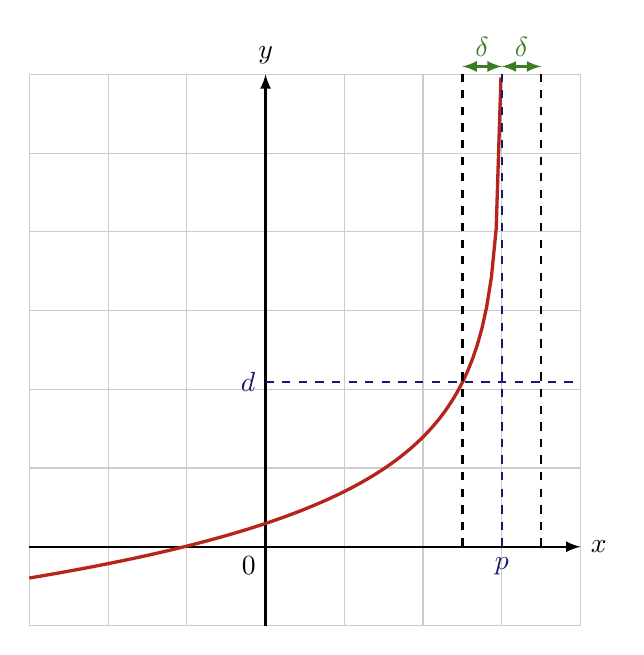
\begin{tikzpicture}
        \draw[thin,gray!40] (-3,-1) grid (4, 6);
        \draw[thick, ->, >=latex] (-3,0)--(4,0) node[right]{\(x\)};
        \draw[thick, ->, >=latex] (0,-1)--(0,6) node[above]{\(y\)};
        \draw (0, 0) node[below left] {0};

        \draw [BrickRed, very thick, domain=-3:2.99, samples=100] plot (\x, {6-ln(300-100*\x)}); 

        \draw[dashed, thick] (2.5, 0) -- (2.5, 6);
        \draw[dashed, thick] (3.5, 0) -- (3.5, 6);
        \draw[MidnightBlue, dashed, thick] (0, 2.09) node[left]{\(d\)} -- (4, 2.09);

        \draw[MidnightBlue, thick, dashed] (3, 0) node[below]{\(p\)} -- (3, 6);

        \draw[OliveGreen, thick, latex-latex, shift={(0, 0.1)}] (2.5, 6) -- (3, 6) node[pos=0.5, above] {\(\delta\)};

        \draw[OliveGreen, thick, latex-latex, shift={(0, 0.1)}] (3, 6) -- (3.5, 6) node[pos=0.5, above] {\(\delta\)};
    \end{tikzpicture}
    
    \caption{As \(x\) approaches \(p\), \(f(x)\) approaches infinity.}
    \label{fig:Ch02-lim-val-inf}
\end{figure}


Now let us consider the opposite scenario where \(L\) is finite but \(p\) is infinite. We modify our definition like so.
%
\begin{quote}
    \textbf{Definition of a limit, with \(p\) infinite and \(L\) finite.}

    The main idea is that \(f(x)\) can become arbitrarily close to \(L\) as long as \(x\) is large enough.

    In other words, {\color{BrickRed} no matter how close we want our output to be to \(L\)}, {\color{Fuchsia} we can always find a value \(c\)} such that {\color{Fuchsia} as long as \(x\) is greater than \(c\)}, {\color{MidnightBlue} the output is within that range}. This is written as
    %
    \[
    {\color{BrickRed}\forall \epsilon > 0},\;
    {\color{Fuchsia} \exists c > 0},\;
    {\color{Fuchsia} \forall x \in \mathbb{R}},\;
    {\color{Fuchsia} x > c}
    \Rightarrow
    {\color{MidnightBlue} \abs{f(x) - L} < \epsilon}
    \text{.}
    \]
\end{quote}
%
See figure \ref{fig:Ch02-lim-inf-val}.


\begin{figure}[H]
    \centering

    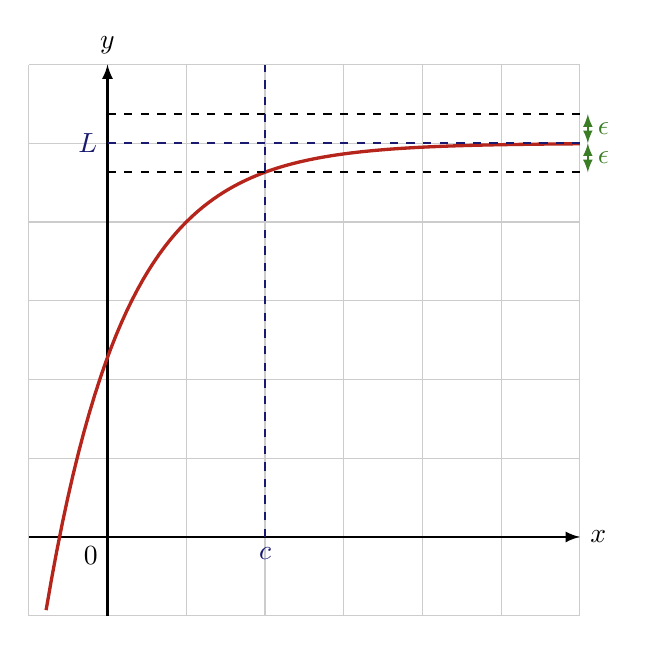
\begin{tikzpicture}
        \draw[thin,gray!40] (-1,-1) grid (6, 6);
        \draw[thick, ->, >=latex] (-1,0)--(6,0) node[right]{\(x\)};
        \draw[thick, ->, >=latex] (0,-1)--(0,6) node[above]{\(y\)};
        \draw (0, 0) node[below left] {0};

        \draw [BrickRed, very thick, domain=-0.78:6, samples=100] plot (\x, {5-2.71828^(1-\x)}); 

        \draw[dashed, thick] (0, 4.63) -- (6, 4.63);
        \draw[dashed, thick] (0, 5.37) -- (6, 5.37);
        \draw[MidnightBlue, dashed, thick] (2, 0) node[below]{\(c\)} -- (2, 6);

        \draw[MidnightBlue, thick, dashed] (0, 5) node[left]{\(L\)}-- (6, 5);

        \draw[OliveGreen, semithick, latex-latex, shift={(0.1, 0)}] (6, 5.37) -- (6, 5) node[pos=0.5, right] {\(\epsilon\)};

        \draw[OliveGreen, semithick, latex-latex, shift={(0.1, 0)}] (6, 5) -- (6, 4.63) node[pos=0.5, right] {\(\epsilon\)};
    \end{tikzpicture}
    
    \caption{As \(x\) approaches infinity, \(f(x)\) approaches \(L\).}
    \label{fig:Ch02-lim-inf-val}
\end{figure}



The final case is where both \(p\) and \(L\) are infinite. The definition for this is as follows.
%
\begin{quote}
    \textbf{Definition of a limit, with both \(p\) and \(L\) infinite.}

    The main idea is that \(f(x)\) can become arbitrarily large as \(x\) gets large enough.

    In other words, {\color{BrickRed} for any value \(d\)}, {\color{Fuchsia} we can always find a value \(c\)} such that {\color{Fuchsia} as long as \(x\) is greater than \(c\)}, {\color{MidnightBlue} the output is greater than \(d\)}. This is written as
    %
    \[
    {\color{BrickRed} \forall d > 0},\;
    {\color{Fuchsia} \exists c > 0},\;
    {\color{Fuchsia} \forall x \in \mathbb{R}},\;
    {\color{Fuchsia} x > c}
    \Rightarrow
    {\color{MidnightBlue} f(x) > d}
    \text{.}
    \]
\end{quote}

See figure \ref{fig:Ch02-lim-inf-inf}.


\begin{figure}[H]
    \centering

    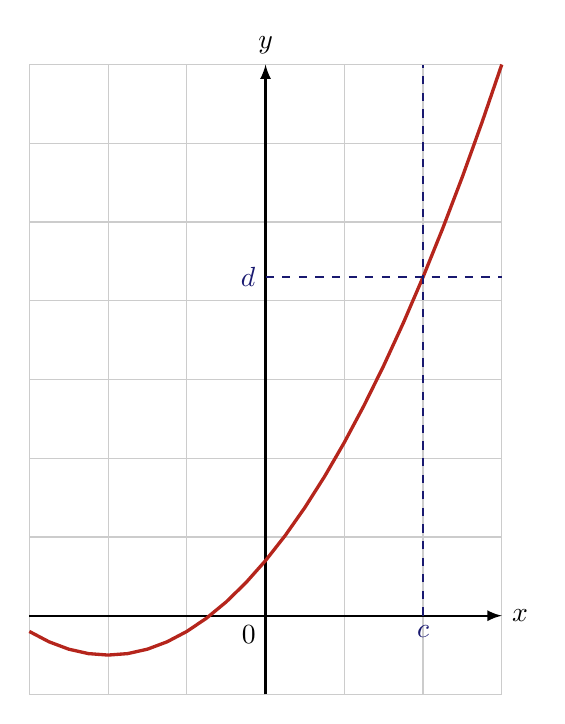
\begin{tikzpicture}
        \draw[thin,gray!40] (-3,-1) grid (3, 7);
        \draw[thick, ->, >=latex] (-3,0)--(3,0) node[right]{\(x\)};
        \draw[thick, ->, >=latex] (0,-1)--(0,7) node[above]{\(y\)};
        \draw (0, 0) node[below left] {0};

        \draw [BrickRed, very thick, domain=-3:3] plot (\x, {0.3*(\x + 2)^2 - 0.5}); 

        \draw[MidnightBlue, dashed, thick] (2, 0) node[below]{\(c\)} --(2, 7);
        \draw[MidnightBlue, dashed, thick] (0, 4.3) node[left]{\(d\)} -- (3, 4.3);
    \end{tikzpicture}
    
    \caption{As \(x\) approaches infinity, so does \(f(x)\).}
    \label{fig:Ch02-lim-inf-inf}
\end{figure}



\subsection{Handling infinities and indeterminate forms}

A limit that exists is known as a \textit{finite} limit. Finite limits can be combined in a natural way.
%
\begin{align*}
    \lim_{x \rightarrow a} (f(x) + g(x)) &= \lim_{x \rightarrow a} f(x) + \lim_{x \rightarrow a} g(x)\\
    \lim_{x \rightarrow a} (f(x) \cdot g(x)) &= \lim_{x \rightarrow a} f(x) \cdot \lim_{x \rightarrow a} g(x)\\
    \lim_{x \rightarrow a} \frac{f(x)}{g(x)} &= \frac{\lim_{x \rightarrow a} f(x)}{\lim_{x \rightarrow a} g(x)}
\end{align*}

We use the following rules to handle infinities.
%
\begin{align*}
    a \times \infty &= \infty\\
    \frac{a}{\infty} &= 0
\end{align*}

If a limit involves \(x\) approaching zero, we may sometimes have to specify the direction in which \(x\) is approaching it, i.e. whether it is approaching zero as a positive number (from the right) or as a negative number (from the left).
%
\begin{align*}
    \lim_{x \rightarrow 0^+} \frac{1}{x} &= \infty\\
    \lim_{x \rightarrow 0^-} \frac{1}{x} &= -\infty
\end{align*}

There are certain cases where we \textit{cannot} combine limits. These are called \textit{indeterminate forms}, and there is no general rule for figuring out what these indeterminate forms evaluate to. Examples of indeterminate forms are given below.
%
\[
\frac{0}{0},\; \frac{\infty}{\infty},\; 0 \times \infty,\; \infty - \infty,\; 0^0,\; 1^\infty,\; \infty^0
\]



\subsection{Little o and big O notation}

It is often useful to talk about the rate at which some function changes as its input increases (or decreases), without worrying to much about the detailed form. To do this, we introduce two types of notation: little \(o\) and big \(O\).

To compare the order of growth of two functions \(f(x)\) and \(g(x)\), we can look at the ratio of the two functions as their input approaches infinity, i.e.
%
\[\lim_{x \rightarrow \infty} \left|\frac{f(x)}{g(x)}\right|\text{.}\]
%
Let's look at how this limit behaves for different functions.


\begin{figure}[H]
    \centering

    \begin{tikzpicture}[scale=0.8]
        \draw[thin,gray!40] (-1,-1) grid (14, 8);
        \draw[thick, ->, >=latex] (-1,0)--(14,0) node[right]{\(x\)};
        \draw[thick, ->, >=latex] (0,-1)--(0,8) node[above]{\(y\)};
        \draw (0, 0) node[below left] {0};

        \draw [BrickRed, very thick, domain=0:14] plot (\x, {0.6*\x-1});
        \draw node[BrickRed] at (9.5, 6) {\(f_1(x) = 0.6x - 1\)};

        \draw [MidnightBlue, very thick, domain=0:14] plot (\x, {0.4*\x+0.5});
        \draw node[MidnightBlue] at (12, 4.25) {\(g(x) = 0.4x - 0.5\)};

        \draw[BurntOrange, very thick, domain=0:14, samples=100] plot (\x, {abs((0.6*\x-1)/(0.4*\x+0.5))});
        \draw node[BurntOrange] at (12, 2) {\(\left|\dfrac{f_1(x)}{g(x)}\right|\)};
    \end{tikzpicture}
    
    \caption{Graphs of a linear function \(f_1(x)\), another linear function \(g(x)\) and the absolute value of their quotient \(|f(x)/g(x)|\).}
    \label{fig:Ch02-linear-linear-quotient-graph}
\end{figure}


Figure \ref{fig:Ch02-linear-linear-quotient-graph} shows the graphs of two functions \(f_1(x) = 0.6x - 1\) and \(g(x) = 0.4x + 0.5\). Both of these functions are linear, so they should have the same order of growth. When this happens, the limit of the ratio of the two functions, as \(x\) approaches infinity, should be a finite constant. As we see in the graph, this is indeed the case, with the orange curve converging to a value of \(1.5\).

Now consider the logarithmic function \(f_2(x) = \ln{x}\) and its relationship with \(g(x)\). As shown in figure \ref{fig:Ch02-log-linear-quotient-graph}, the limit of their ratio once again converges to a finite constant: zero. This is because the logarithmic function grows much slower than the linear function.

\begin{figure}[H]
    \centering

    \begin{tikzpicture}[scale=0.8]
        \draw[thin,gray!40] (-1,-1) grid (14, 8);
        \draw[thick, ->, >=latex] (-1,0)--(14,0) node[right]{\(x\)};
        \draw[thick, ->, >=latex] (0,-1)--(0,8) node[above]{\(y\)};
        \draw (0, 0) node[below left] {0};

        \draw [BrickRed, very thick, domain=0.375:14, samples=100] plot (\x, {ln(\x)});
        \draw node[BrickRed] at (12.5, 3) {\(f_2(x) = \ln{x}\)};

        \draw [MidnightBlue, very thick, domain=0:14] plot (\x, {0.4*\x+0.5});
        \draw node[MidnightBlue] at (12, 4.25) {\(g(x) = 0.4x - 0.5\)};

        \draw[BurntOrange, very thick, domain=0.02:14, samples=100] plot (\x, {abs(ln(\x)/(0.4*\x+0.5))});
        \draw node[BurntOrange] at (12, 1.25) {\(\left|\dfrac{f_2(x)}{g(x)}\right|\)};
    \end{tikzpicture}
    
    \caption{Graphs of a logarithmic function \(f_2(x)\), a linear function \(g(x)\) and the absolute value of their quotient \(|f(x)/g(x)|\).}
    \label{fig:Ch02-log-linear-quotient-graph}
\end{figure}

From this we can gather that the limit of the ratio of two functions \(f(x)\) and \(g(x)\) is bounded (i.e. a finite constant) when \(f(x)\) grows \textit{as fast as} or \textit{slower} than \(g(x)\). We can denote this with big \(O\) notation, as \(f(x) = O(g(x))\). The definition of big \(O\) notation is given below.
%
\begin{quote}
    \textbf{Big \(\mathbf{O}\) notation.}

    We write \(f = O(g)\) near infinity if \(\lim_{x \rightarrow \infty} \left|\frac{f(x)}{g(x)}\right|\) is bounded, i.e.
    %
    \[\exists M \in \mathbb{R},\; \lim_{x \rightarrow \infty} \left|\frac{f(x)}{g(x)}\right| < M\text{.}\]
    
    Sometimes we want to consider the growth rate of functions not just near infinity but near a specific point \(x = b\). In this case, we write \(f = O(g)\) near \(b\) if
    %
    \[\exists M \in \mathbb{R},\; \lim_{x \rightarrow b} \left|\frac{f(x)}{g(x)}\right| < M\text{.}\]
\end{quote}

Remember that big \(O\) notation covers two cases:
%
\begin{itemize}
    \item \(f(x)\) grows as fast as \(g(x)\) (meaning that the two functions have the same order of growth), or
    \item \(f(x)\) grows slower than \(g(x\)) (meaning that the former has a lower order of growth than the latter).
\end{itemize}
%
If we want to be more specific and consider only the second case where \(f(x)\) grows strictly slower than \(g(x)\), we can use little \(o\) notation to write \(f(x) = o(g(x))\). The definition of little \(o\) notation is given below.
%
\begin{quote}
    \textbf{Little \(\mathbf{o}\) notation.}

    We write \(f = o(g)\) near infinity if \(\lim_{x \rightarrow \infty} \frac{f(x)}{g(x)} = 0\).
    
    Again, we sometimes want to consider the growth rate of functions near a specific point \(x = b\). For this we say that \(f = o(g)\) near \(b\) if \(\lim_{x \rightarrow b} \frac{f(x)}{g(x)} = 0\).    
\end{quote}

Note that since little \(o\) is a special case of big \(O\), we have \(f = o(g) \;\Rightarrow\; f = O(g)\).



\subsection{Continuity}

A function \(f\) is continuous if for all \(a\) where \(f(a)\) is defined, we have \(\lim_{x\rightarrow a} f(x) = f(a)\).

In practice, this means that the graph of \(y = f(x)\) is a single unbroken curve. The exponential and logarithm functions, for example, are both continuous.

An important result of this is the \textit{intermediate value theorem}.
%
\begin{quote}
    \textbf{Intermediate value theorem.}

    Assume for a continuous function \(f\) that \(a < b\) and \(f(a) < f(b)\). For any value \(y\) such that \(f(a) < y < f(b)\), there exists a (not necessarily unique) value \(x\) such that \(a < x < b\) and \(f(x) = y\).
\end{quote}
%
See figure \ref{fig:Ch02-int-value-thm} and \ref{fig:Ch02-int-value-thm-uniqueness}.

\begin{figure}[H]
    \centering

    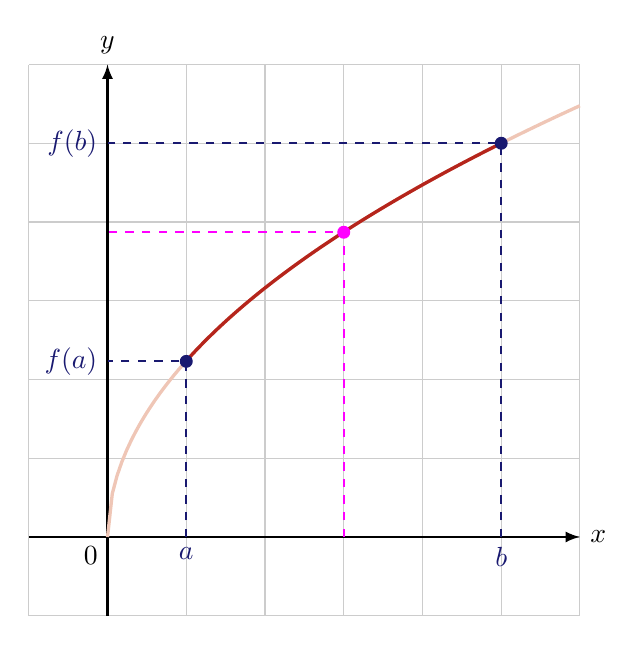
\begin{tikzpicture}
        \draw[thin,gray!40] (-1,-1) grid (6, 6);
        \draw[thick, ->, >=latex] (-1,0)--(6,0) node[right]{\(x\)};
        \draw[thick, ->, >=latex] (0,-1)--(0,6) node[above]{\(y\)};
        \draw (0, 0) node[below left] {0};

        \draw [BrickRed!20, very thick, domain=0:6, samples=100] plot (\x,
        {sqrt(5*\x)});

        \draw [BrickRed, very thick, domain=1:5, samples=100] plot (\x,
        {sqrt(5*\x)});

        \filldraw[radius=0.075, MidnightBlue] (1, 2.23) circle;
        \draw[dashed, MidnightBlue, thick] (1, 0) node[below]{\(a\)} -- (1, 2.23) -- (0, 2.23) node[left]{\(f(a)\)};

        \filldraw[radius=0.075, Fuchsia] (3, 3.87) circle;
        \draw[dashed, Fuchsia, thick] (3, 0) -- (3, 3.87) -- (0, 3.87);


        \filldraw[radius=0.075, MidnightBlue] (5, 5) circle;
        \draw[dashed, MidnightBlue, thick] (5, 0) node[below]{\(b\)} -- (5, 5) -- (0, 5) node[left]{\(f(b)\)};
    \end{tikzpicture}
    
    \caption{The intermediate value theorem.}
    \label{fig:Ch02-int-value-thm}
\end{figure}


\begin{figure}[H]
    \centering

    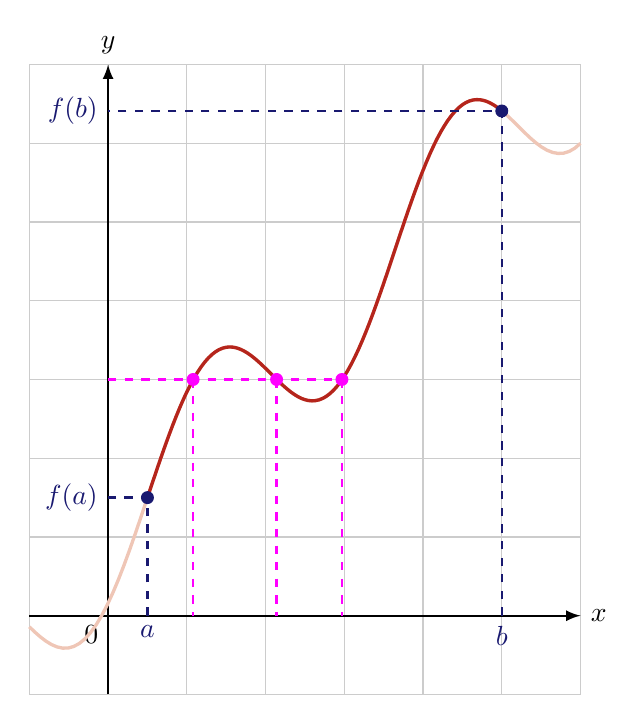
\begin{tikzpicture}
        \draw[thin,gray!40] (-1,-1) grid (6, 7);
        \draw[thick, ->, >=latex] (-1,0)--(6,0) node[right]{\(x\)};
        \draw[thick, ->, >=latex] (0,-1)--(0,7) node[above]{\(y\)};
        \draw (0, 0) node[below left] {0};

        \draw [BrickRed!20, very thick, domain=-1:6, samples=100] plot (\x,
        {sin((2*\x-1) r)+\x+1});

        \draw [BrickRed, very thick, domain=0.5:5, samples=100] plot (\x,
        {sin((2*\x-1) r)+\x+1});

        \filldraw[radius=0.075, MidnightBlue] (0.5, 1.5) circle;
        \draw[dashed, MidnightBlue, thick] (0.5, 0) node[below]{\(a\)} -- (0.5, 1.5) -- (0, 1.5) node[left]{\(f(a)\)};

        \filldraw[radius=0.075, Fuchsia] (1.08, 3) circle;
        \draw[dashed, Fuchsia, thick] (1.08, 3) -- (1.08, 0);
        \filldraw[radius=0.075, Fuchsia] (2.14, 3) circle;
        \draw[dashed, Fuchsia, thick] (2.14, 3) -- (2.14, 0);
        \filldraw[radius=0.075, Fuchsia] (2.97, 3) circle;
        \draw[dashed, Fuchsia, thick] (2.97, 3) -- (2.97, 0);

        \draw[dashed, Fuchsia, thick] (0, 3) -- (2.97, 3);

        \filldraw[radius=0.075, MidnightBlue] (5, 6.41) circle;
        \draw[dashed, MidnightBlue, thick] (5, 0) node[below]{\(b\)} -- (5, 6.41) -- (0, 6.41) node[left]{\(f(b)\)};
    \end{tikzpicture}
    
    \caption{In the intermediate value theorem, for a given value \(y\), the value of \(x\) does not necessarily have to be unique.}
    \label{fig:Ch02-int-value-thm-uniqueness}
\end{figure}